\section{Teoría del flujo unidimensional}


\subsection{Sistema y volumen de control}

\subsubsection{Sistema de control}
Un sistema de control se refiere a una masa fija (infinitesimal o finita) definida y se distingue de todas las demás. Las fronteras del sistema forman una superficie cerrada. Esta superficie puede variar en el tiempo de tal manera que mantenga la misma masa durante los cambios. Es decir $dm/dt = 0$.
En el enfoque \emph{Lagrangiano} en el cual el estudio se centra en el movimiento de partículas individuales, el movimiento se observa como una función del tiempo. Es decir se "sigue" a la partícula, como en el estudio de sólidos. En este caso se utiliza un sistema de control, ya que la masa de la partícula o solido se mantiene constante

\subsubsection{Volumen de control}
En el enfoque \emph{Euleriano} se mantiene fija la coordenada espacial y así se pueden observar las velocidades de las partículas móviles al pasar por esta posición en cualquier instante. Entonces, las propiedades del flujo son funciones del espacio y el tiempo.
Este tipo de enfoque se puede estudiar a través de un volumen de control o punto fijo, en el cual el flujo pasa a traces de este.

%%%%%%%%%%%%%%%%%%%%%%%%%%%%%%%%%%%%%%%%%%%%%%%%%%%%%%
\subsection{Linea y tubo de corriente}

\subsubsection{Linea de trayectoria}
Es el lugar geométrico de los puntos recorridos por una partícula determinada cuando se desplaza en un campo de flujo.

\subsubsection{Linea de corriente}
Es una línea continua que representa el flujo y ésta posee la propiedad de que el vector velocidad de cada partícula es tangente a la línea de corriente. La ecuacion que representa el vector: $ \overline{v} x d\overline{r} = 0$

\begin{figure}[h]
	\centering
	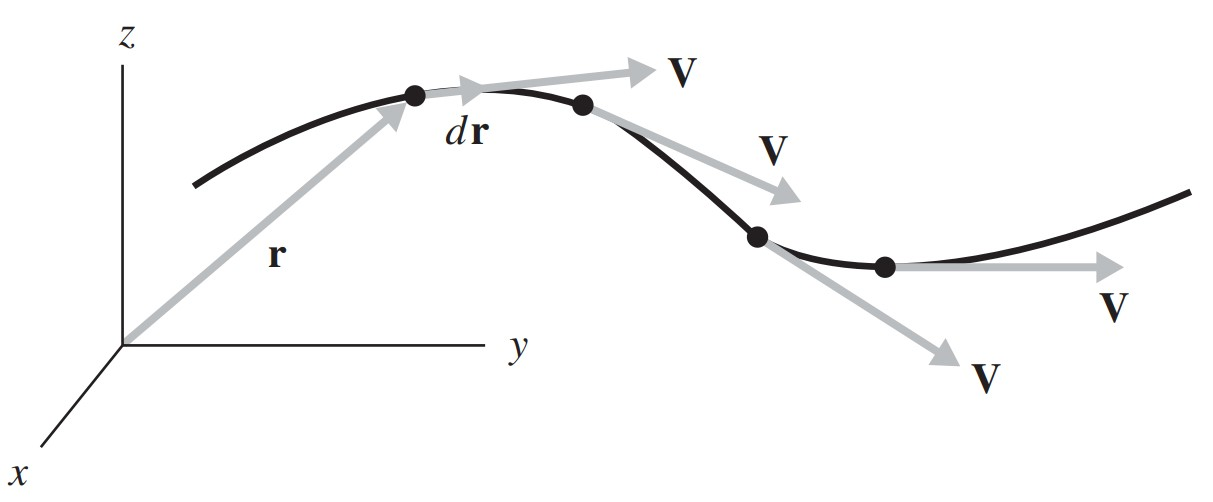
\includegraphics[width = .5\linewidth]{U3-linea-corriente}
	\caption{Linea de corriente en un campo de flujo}
\end{figure}

En un flujo \emph{permanente} la trayectoria de una partícula es una linea de corriente. Pero en un flujo no permanente donde el vector velocidad cambia con el tiempo, haciendo que la partícula siga diferentes lineas de corrientes de tal manera que la trayectoria de esta no puede parecerse a ninguna linea de corriente.

\subsubsection{Tubo de corriente}
Un tubo de corriente está constituido por una región parcial del flujo delimitada por una familia de lineas de corriente. No existe flujo a través de las paredes ya que el vector velocidad no tiene componete perpendicular a la superficie del tubo ya que siempre es tangente a la linea de corriente.

%%%%%%%%%%%%%%%%%%%%%%%%%%%%%%%%%%%%%%%%%%%%%%%%%%%%%%%%%%%%%%%
\subsection{Tipos de flujo}
\subsubsection{Flujo permanente}
Ocurre cuando las condiciones en cualquier punto del fluido no cambian con el tiempo es decir:

\begin{tabular}{r c l}
	$\dfrac{\delta v}{\delta t} = 0$ & $\dfrac{\delta p}{\delta t}$ & $ \dfrac{\delta \rho}{\delta t}$
\end{tabular}

Esto no significa que la velocidad no varíe de un punto.

\subsubsection{Flujo en una, dos y tres dimensiones}

\subsubsection{Flujo laminar y turbulento}
En un \textbf{flujo laminar} las partículas se mueven a lo largo de trayectorias suaves en láminas o capas, con una capa deslizándose suavemente sobre otra adyacente. El flujo laminar está gobernado por la ley de viscosidad de Newton, la cual relaciona el esfuerzo cortante con la tasa de deformación angular. En situaciones de baja viscosidad, alta velocidad o grandes caudales, este flujo no es estable y se rompe en flujo turbulento.\\

En un \textbf{flujo turbulento} los movimientos del fluido varían irregularmente. Las partículas se mueven en trayectorias arremolinadas causando un intercambio de momentum. La turbulencia causa mayores esfuerzos cortantes y pérdidas.\\

Si un flujo es laminar o turbulento depende de tres parámetros físicos que combinados forman el número de \textbf{Reynolds} y nos permite determinar el régimen de flujo:\\

\begin{tabular}{c c}
		\begin{minipage}[t]{.45\textwidth}
			\flushright 
			\vspace{.05cm}
			$Re= \dfrac{V L}{\nu}$
		\end{minipage}
		&
		\begin{minipage}[t]{.45\textwidth}
			\flushleft
			V velocidad\\
			L Longitud\\
			$\nu$ viscosidad cinemática
		\end{minipage}
\end{tabular}

\subsubsection{Flujos viscosos e inviscidos}
\subsubsection{Flujo compresible e incompresible}
		



%%%%%%%%%%%%%%%%%%%%%%%%%%%%%%%%%%%%%%%%%%%%%%%%%%%%%%%%%%%%
